\documentclass[12pt]{article}
\usepackage[longnamesfirst]{natbib}
\usepackage{amssymb}

% \usepackage{color} option clash
\usepackage{graphicx}
% \usepackage[dvips]{graphics}

% \input{../standard}

%%%%%  standard

\renewcommand{\baselinestretch}{1.4} 

\setlength{\abovedisplayskip 0.1in}
\setlength{\belowdisplayskip 0.1in}

\newcommand{\iid}{\stackrel {\mbox{\scriptsize iid}}{\sim}}
\newcommand{\pr}{\mbox{P}}
\newcommand{\fdr}{\mbox{\it FDR}}

\newtheorem{lemma}{Lemma}
\newtheorem{theorem}{Theorem}
\newtheorem{corollary}[theorem]{Corollary}
\newtheorem{claim}[theorem]{Claim}
\newtheorem{defn}{Definition}[section]
\newtheorem{cor}[theorem]{Corollary}

\newcommand{\be}{\begin{equation}}
\newcommand{\qe}[1]{\label{#1}\end{equation}}

\newcommand{\sumall}{\sum_{j=1}^{\infty}}
\newcommand{\sumzi}[1] {\sum_{#1=0}^{\infty}}
\newcommand{\sumii}[1] {\sum_{#1=-\infty}^{\infty}}
\newcommand{\piint}{\int_{-\pi}^{\pi}}
\newcommand{\pimint}{\int_{(-\pi,\pi]}}
\newcommand{\pipint}{\int_{(-\pi,\pi]}}
\newcommand{\tr}{\mbox{tr}}

\newcommand{\cov}{\,\mbox{cov}}
\newcommand{\corr}{\,\mbox{corr}}
\newcommand{\var}{\,\mbox{var}}
\newcommand{\cum}{\,\mbox{cum}}
\newcommand{\Cov}{\,\mbox{Cov}}
\newcommand{\Corr}{\,\mbox{Corr}}
\newcommand{\Var}{\,\mbox{Var}}
\newcommand{\Cum}{\,\mbox{Cum}}

% Journals, as abbreviated in bibtex
\newcommand{\AS}{Annals of Statistics}
\newcommand{\IEEEIT}{IEEE Trans. on Info. Theory}
\newcommand{\JASA}{Journal of the Amer. Statist. Assoc.}
\newcommand{\JBES}{Journal of Bus. and Econ. Statist.}
\newcommand{\JRSSA}{Journal of the Royal Statist. Soc., Ser. A}
\newcommand{\JRSSB}{Journal of the Royal Statist. Soc., Ser. B}
\newcommand{\JTS}{Journal of Time Series Analysis}
\newcommand{\TAS}{The American Statistician}
\newcommand{\StatSci}{Statistical Science}

% Convergence symbols
\newcommand{\as}{\stackrel{\mbox{\scriptsize  a.s.}}{\rightarrow}}
\newcommand{\inp}{\stackrel{\mbox{\scriptsize P}}{\rightarrow}}

% Symbol two-letter abbreviations
\newcommand{\al}{\alpha}
\newcommand{\bt}{\beta}
\newcommand{\ep}{\epsilon}
\newcommand{\ga}{\gamma}
\newcommand{\la}{\lambda}

% fractions
\newcommand{\half}{\mbox{$\frac{1}{2}$}}
\newcommand{\third}{\mbox{$\frac{1}{3}$}}
\newcommand{\quarter}{\mbox{$\frac{1}{4}$}}
\newcommand{\smfrac}[2]{\mbox{$\frac{\scriptstyle #1}{\scriptstyle #2}$}}
\newcommand{\smquarter}{\smfrac{1}{4}}
\newcommand{\smhalf}{\smfrac{1}{2}}

% Miscellaneous
\newcommand{\eqn}[1]{(\ref{#1})}
% \newcommand{\implies}{\quad \Rightarrow \quad}
\newcommand{\given}{\; \big| \;}
% \newcommand{\iff}{\quad \Leftrightarrow \quad}
\newcommand{\QED}{\frame{\rule{0pt}{6pt}\rule{6pt}{0pt}}}
% \newcommand{\qed}{\hfill $\Box$}


\newcommand{\osb}[1]{1_{\{#1\}}}
\newcommand{\rone}{R^{1}}
\newcommand{\rn}{R^{n}}
\newcommand{\rfty}{R^{\infty}}
\newcommand{\nv}{^{\leftarrow}}
\newcommand{\ap}{\rightarrow}
\newcommand{\apty}{\ap\infty}
\newcommand{\nd}{\mbox{\hspace{12pt}}}
\newcommand{\ve}[1]{\underline{\underline{#1}}}
\newcommand{\sgsq}{\sigma^2}
\newcommand{\cid}{\Rightarrow}
\newcommand{\ul}[1]{\underline{#1}}
\newcommand{\ol}[1]{\overline{#1}}
\newcommand{\asdt}{\mbox{ as }dt\ap 0}

%------------------------------------------------------------------------eof

\newtheorem{definition}{Definition}
\newtheorem{example}{Example}

% --- Paragraph split
\setlength{\parskip}{0.00in}

% --- Line spacing
\renewcommand{\baselinestretch}{1.4}

% --- Margin notes on the left-hand-side
%    \marginpar{\scriptsize\raggedright note}
\setlength{\topmargin}{0in}         % 1.5 in top/bottom
\setlength{\headheight}{0.25in}
\setlength{\headsep}{0.25in}
\setlength{\textheight}{8.0in}
\setlength{\oddsidemargin}{0.0in}   % 1. in left/right
\setlength{\textwidth}{6.5in}

% --- Hypthenation
\sloppy  % fewer hyphenated
\hyphenation{stan-dard}
\hyphenation{among}

% --- Customized commands, abbreviations
\newcommand{\TIT}{{\it  {\tiny  Alpha-investing}}}
\newcommand{\SDR}[1]{{\mbox{$\mbox{SDR}_{\mbox{\scriptsize #1}}$}}}

% --- Header
\pagestyle{myheadings}
\markright{\TIT}

\usepackage[usenames]{color}

\newcommand{\jrss}[1]{\noindent{\textcolor{red}{\{{\bf jrss:} \em
#1\}}}}
\newcommand{\dpf}[1]{\noindent{\textcolor{blue}{\{{\bf dpf:} \em
#1\}}}}
\newcommand{\ras}[1]{\noindent{\textcolor{green}{\{{\bf ras:} \em
#1\}}}}


% --- Title

\title{  
\vspace{-0.5em}
         Alpha-investing: A  procedure for sequential control of
                                   expected false discoveries 
\vspace{-0.5em}
}
% \title{  
%        Multiple hypothesis testing using \\
%        the excess discovery count and alpha-investing rules
% }

\author{
        Dean P. Foster and Robert A. Stine\footnote{All correspondence
regarding this manuscript should be directed to Prof. Stine at 
the address shown with the title.  He can be reached via e-mail at
stine@wharton.upenn.edu.}                                    \\
        Department of Statistics                             \\
        The Wharton School of the University of Pennsylvania \\
        Philadelphia, PA 19104-6340                          \\
}

\date{\today}
% \date{April 7, 2005}

%%%%%%%%%%%%%%%%%%%%%%%%%%%%%%%%%%%%%%%%%%%%

\begin{document}
\maketitle 
%------------------------------------------------------------------------
\vspace{-2em}

\abstract{ 
\vspace{-0.5em}
 Alpha-investing is an adaptive, sequential methodology that encompasses a large family of procedures  for testing multiple hypotheses. All control mFDR, which is the ratio of
 the expected number of false rejections to the expected number of
 rejections. mFDR is a weaker criterion than FDR, which is the
 expected value of the ratio.  We compensate for this weakness by
 showing that alpha-investing controls mFDR at every rejected
 hypothesis.  Alpha-investing resembles alpha-spending used
 in sequential trials, but possesses a key difference.  When a test
 rejects a null hypothesis, alpha-investing earns additional
 probability toward subsequent tests.  Alpha-investing hence allows one
 to incorporate domain knowledge into the testing procedure and
 improve the power of the tests. In this way, alpha-investing
 enables the statistician to design a testing procedure for a specific problem 
 while guaranteeing control of mFDR.  }

%------------------------------------------------------------------------
\vspace{0.05in}

\noindent
{\it Key words and phrases: 
  alpha spending,
  Bonferroni method,
  false discovery rate (FDR, mFDR), 
  family-wise error rate (FWER),
  multiple comparisons.
}


 
% ----------------------------------------------------------------------
\section{Introduction}                                   %  1
% ----------------------------------------------------------------------
\label{sec:introduction}

We propose an adaptive, sequential methodology for testing multiple
hypotheses. Our approach, called alpha-investing, works in the usual
setting in which one has a batch of several hypotheses as well as in
cases in which hypotheses arrive sequentially in a stream.
Streams of hypotheses arise naturally in  contemporary
modeling applications such as genomics and variable selection for
large models.  In contrast to the comparatively small problems that
spawned multiple comparison procedures, modern applications can
involve thousands of tests.  For example, micro-arrays lead one to
compare a control group to a treatment group using measured
differences on over 6,000 genes \citep{shaffer03}.  If one considers
the possibility for interactions, then the number of tests is
virtually infinite. In contrast, the example used by Tukey to motivate
multiple comparisons compares the means of only 6 groups
\citep[][available in \citet{braun94}] {tukey53}.  Because
alpha-investing tests hypotheses sequentially, the choice
of future hypotheses can depend upon the results of previous tests.
Thus, having discovered differences in certain genes, an investigator
could, for example, direct attention toward genes that share common
transcription factor binding sites \citep{gupta05}. \citet{wasserman06} 
describes other testing situations that offer domain knowledge.

Before we describe alpha-investing, we introduce a variation on
 the marginal false discovery rate (mFDR), an existing criterion for
 multiple testing.  Let the observable
 random variable $R$ denote the total number of hypotheses rejected by
 a testing procedure, and let $V$ denote the unobserved number of
 falsely rejected hypotheses.  A testing procedure controls mFDR
 at level $\alpha$ if
\begin{equation}
\label{eq:mFDR}
\hbox{mFDR}_1 \equiv \frac{E(V)}{E(R) + 1} \le \alpha.
\end{equation}
mFDR traditionally does not add 1 to the denominator; following our
notation, we denote the traditional version mFDR${}_0$. 
The addition of a positive constant to the denominator
avoids statistical problems under the complete null hypothesis.  Under the
complete null hypothesis, all hypotheses are false, implying, $V \equiv R$
and mFDR${}_{0}$ = 1. 


An alpha-investing rule is an adaptive testing procedure that
resembles an alpha-spending rule.  An
alpha-spending rule begins with an allowance for Type I error,
what we call the initial alpha-wealth of the procedure.  Each test at
level $\alpha_i$ reduces the alpha-wealth  by
$\alpha_i$.  Once the alpha-wealth of the spending rule reaches zero,
no further tests are allowed.  Because the total chance
for a Type I error is bounded by the initial alpha-wealth,
alpha-spending naturally implements a Bonferroni rule. For
multiple testing, however, Bonferroni rules are too conservative.  
An alpha-investing rule overcomes this conservatism by earning 
a contribution to its alpha-wealth for each rejected null hypothesis.  
Thus rejections beget more rejections.  Alpha-investing rules further
allow one to test an infinite stream of hypotheses, accommodate dependent tests, and incorporate domain knowledge, all the while controlling mFDR.


The sequential nature of alpha-investing allows us to enhance the
 type of control obtained through mFDR.  By placing mFDR in a sequential setting, we can require that a testing procedure does well if stopped early.  
 Suppose rather than testing all
 $m$ hypotheses, the statistician stops after rejecting 10.
  We would like to be able to assure her that no more than, say, 2 of
 these were false rejections, on average.  This further protection  distinguishes
 what we call uniform control of mFDR. We show that alpha-investing uniformly controls
 mFDR.  
 
 In general,
suppose we test hypotheses until the number of rejections $R$
reaches some target $r$.  Let $T_{r}$ identify the index of this test.
Define $V(T_{r})$ to be the number of nulls that have been incorrectly
rejected at this point. A test procedure uniformly controls
mFDR${}_{1}$ if this stopped process controls mFDR${}_{1}$ in the
sense of (\ref{eq:mFDR}). In words, equation (\ref{eq:mFDR}) implies
that the expected value of $V$ given that $R=r$ is less than or
equal to $\alpha(r+1)$.  This conditional expectation requires that we
introduce a stopping time.  We defer these details to Section \ref{sec:sFDR}.  As a
preview, we offer
\begin{theorem}\label{thm:stopped}
An alpha-investing rule with control parameters set to $\alpha$ has
 the property that $E \; V(T_{r}) \le \alpha(r+1)$ where $T_{r}$ is
 the stopping time defined by occurrence of the $r^{th}$ rejection and
 $V(m)$ is the number of false rejections among tests of $m$ hypotheses.
\end{theorem}

The rest of this paper develops as follows.  We first review several
 ideas from the literature on multiple comparisons, particularly those
 related to the family-wise error rate and false discovery rate (FDR).  
 Next we discuss alpha-investing rules in Section \ref{sec:alpha:investing}.  In
 Sections \ref{sec:mFDR} and \ref{sec:sFDR} we discuss uniform control
 of mFDR.  We describe the design and performance of
 alpha-investing rules  in Section
 \ref{sec:examples}.  We close in Section \ref{sec:discussion} with a
 brief discussion. 


%--------------------------------------------------------------------------
\section{Criteria and Procedures }  \label{sec:procedure} % 2
%--------------------------------------------------------------------------

Suppose that we have  $m$ null hypotheses ${\cal H}(m) =
\{H_1, \, H_2, \ldots, H_m\}$ that specify values for parameters
$\theta = \{\theta_1,\,\theta_2, \ldots, \theta_m \}$.  Each parameter
$\theta_j$ can be scalar or vector-valued, and $\Theta$ denotes the
space of parameter values.  In the most familiar case, each null
hypothesis specifies that a scalar parameter is zero, $H_j: \theta_j =
0$. 


We follow the standard notation for labeling correct and incorrect
rejections \citep{benjamini95}.  Assume that $m_0$ of the null
hypotheses in ${\cal H}(m)$ are true.  The {\em observable} statistic
$R(m)$ counts how many of these $m$ hypotheses are rejected.   A 
superscript $\theta$ distinguishes {\em unobservable} random variables from 
statistics such as $R(m)$.  The random variable 
$V^\theta(m)$ denotes the number of
false positives among the $m$ tests, counting cases in which the testing
procedure incorrectly rejects a true null hypothesis.  
$S^{\theta}(m) = R(m)-V^\theta(m)$ counts the number of correctly
rejected null hypotheses. Under the complete null hypothesis, 
$m_0 = m$, $V^\theta(m) \equiv R(m)$, and $S^{\theta}(m) \equiv 0$.


The original intent of multiple testing was to control the chance for {\em
any} false rejection.  The {\em family-wise error rate} (FWER) is the
probability of falsely rejecting any null hypothesis from ${\cal
H}(m)$,
\begin{equation}
  \mbox{FWER}(m) \equiv 
   \sup_{\theta \in \Theta} \pr_\theta(V^\theta(m) \ge 1) \;.
\label{eq:fwer}
\end{equation}
An important special case is control of FWER under the complete null
 hypothesis:
$ \pr_0(V^\theta(m) \ge 1) \le \alpha$,
where $\pr_0$ denotes the probability measure under the complete null
 hypothesis.  We refer to  controlling FWER under the complete null hypothesis
 as controlling FWER in the weak sense.


Bonferroni procedures control FWER.  Let $p_1, \ldots, p_m$ denote the p-values
of tests of $H_1, \ldots, H_m$.  Given a chosen level $0 < \alpha < 1$,
the simplest Bonferroni procedure rejects those $H_j$ for which $p_j \le
\al/m$.  Let the indicators $V^\theta_j \in \{0, 1\}$ track incorrect
rejections; $V^\theta_j = 1$ if $H_j$ is incorrectly rejected and is
zero otherwise.  Then $V^\theta(m) = \sum V^{\theta}_{j}$ and the
inequality
\begin{equation}
  \pr_\theta(V^\theta(m) \ge 1) 
     \le \sum_{j=1}^m \pr_\theta(V^{\theta}_{j} = 1) \le \al
\label{eq:Bon}
\end{equation}
shows that this procedure controls
$\mbox{FWER}(m) \le \alpha$.  One need not distribute $\alpha$ equally
over ${\cal H}(m)$; the inequality \eqn{eq:Bon} requires only that the
sum of the $\alpha$-levels not exceed $\alpha$.  This observation
suggests an alpha-spending characterization of the Bonferroni
procedure.  As an alpha-spending rule, the Bonferroni procedure
allocates $\alpha$ over a collection of hypotheses, devoting a larger
share to hypotheses of greater interest.  In effect, the procedure has
a budget of $\alpha$ to spend.  It can spend $\alpha_j \ge 0$ on
testing each hypothesis $H_j$ so long as $\sum_j \alpha_j \le \alpha$.
Although such alpha-spending rules control FWER, they are often
criticized for having little power.  Clearly, the power of the
traditional Bonferroni procedure decreases as $m$ increases because
the threshold $\alpha/m$ for detecting a significant effect decreases.
The testing procedure introduced in \citet{holm79} offers more power
while controlling FWER, but the improvements are small.


To obtain substantially more power,
\citet{benjamini95} (BH) introduces a different criterion, the false
discovery rate (FDR).  FDR is the 
expected proportion of false positives among rejected hypotheses,
\begin{equation}
  \mbox{FDR}(m) = E_\theta \left(\frac{V^\theta(m)}{R(m)} \given R(m)>0 \right)
               \pr (R(m)>0)  \;.
\label{eq:fdr}
\end{equation}
For the complete null hypothesis, 
$\mbox{FDR}(m) = \pr_0(R(m)>0)$, which is $\mbox{FWER}(m)$.
Thus, test procedures that control FDR$(m) \le \alpha$ also control
FWER$(m)$ in the weak sense at level $\alpha$.   If the complete null
 hypothesis is rejected, FDR introduces a different type of control.  
 Under the alternative,
$\mbox{FDR}(m)$ decreases as the number of false null hypotheses
$m-m_0$ increases \citep{shaffer03}.  As a result, $\mbox{FDR}(m)$
becomes more easy to control in the presence of non-zero effects,
allowing more powerful procedures.  Variations on FDR include pFDR
\citep[which drops the term $\pr (R>0)$; see][]{storey02,storey03} and the
local false discovery rate $\mbox{fdr}(z)$ \citep[which estimates the
  false discovery rate as a function of the size of the test
  statistic; see ][]{efron07}.  Closer to our work,
 \citet{meinshausen04b} and \citet{rice06} estimate
$m_0$, the total number of false null hypotheses in ${\cal H}(m)$, 
and \citet{wasserman06} weight p-values based on prior knowledge
that identifies hypotheses that are likely to be false.  \citet{benjamini95} also considers mFDR${}_0$ and mFDR${}_1$, which they considered artificial.  mFDR does not control a property of
 the realized sequence of tests; instead it controls a ratio of
 expectations. 

 
\citet{benjamini95} also introduces a step-down testing procedure that
 controls FDR. Order the collection of $m$ hypotheses so that
 the p-values of the associated tests are sorted from
 smallest to largest (putting the most significant first),
\begin{equation}
  p_{(1)} \le p_{(2)} \le \cdots \le p_{(m)} \;.
\label{eq:ordered:pv}
\end{equation}
The test of $H_{(1)}$ has p-value $p_{(1)}$, the test of $H_{(2)}$ has
p-value $p_{(2)}$, and so forth.  If $p_{(1)} > \alpha/m$, the BH procedure stops
and does not reject any hypothesis.  This step controls FWER  in
the weak sense at level $\alpha$.  If $p_{(1)} \le \alpha/m$, the
procedure rejects $H_{(1)}$ and moves on to $H_{(2)}$.  Rather
than compare $p_{(2)}$ to $\alpha/m$, however, the BH procedure
compares $p_{(2)}$ to $2 \alpha/m$.  In general, the BH
step-down procedure rejects $H_{(1)}, \ldots, \, H_{(j_d - 1)}$ for  
$j_d = \min\{j:p_{(j)} > j\alpha / m\}$.
Clearly this sequence of increasing thresholds obtains more power than 
a Bonferroni procedure.  If
the p-values are independent, the inequality of \citet{simes86}
implies that this step-down procedure satisfies FDR.  This sequence of
thresholds, however, does not control FWER$(m)$ in general.  This is
the price we pay for the improvement in power.  Subsequent papers
\citep[such as][]{benjamini01, sarkar98, troendle96} consider
situations in which the BH procedure controls FDR under certain types
of dependence.

%--------------------------------------------------------------------------
\section{Alpha-Investing Rules}   \label{sec:alpha:investing}         % 3
%--------------------------------------------------------------------------

Alpha-investing resembles alpha-spending
 used in sequential clinical trials.  In a
 sequential trial, investigators perform a sequence
 of tests of one (or perhaps a few) null hypotheses as the data
 accumulate.  An alpha-spending (or error-spending) rule controls the
 level of such tests.  Given an overall Type I error rate, say $\al = 0.05$, 
 an alpha-spending rule allocates, or spends,
 $\alpha$ over a sequence of tests.  As \citet{tukey91} writes, ``Once
 we have spent this error rate, it is gone.''  


While similar in that they allocate Type I error over multiple tests,
 an alpha-investing rule earns additional probability
 toward subsequent Type I errors with each rejected hypothesis.
  Rather than treat each test as an expense that consumes its Type
 I error rate, an alpha-investing rule treats tests as investments,
 motivating our choice of name. An alpha-investing rule earns an increment in its
 alpha-wealth each time that it rejects a null hypothesis.  For alpha-investing, Tukey's remark becomes ``Rules that invest the error rate
 wisely earn more for further tests.''   The more
 hypotheses that are rejected, the more alpha-wealth it earns.  If the
 test of $H_j$ is not significant, however, an alpha-investing rule
 loses the invested  $\alpha$-level.


More specifically, an alpha-investing rule $\cal I$ is a function that
 determines the $\alpha$-level for testing the next hypothesis in a
 sequence of tests.  We assume an exogenous system external to the
 investing rule chooses which hypothesis to test next.  (Though not
 part of the investing rule itself, this exogenous system can use the
 sequence of rejections to pick the next hypothesis.) 
 Let $W(k) \ge 0$ denote the alpha-wealth accumulated by an
 investing rule after $k$ tests; $W(0)$ is the initial alpha-wealth.
 Conventionally, $W(0) = 0.05$ or $0.10$.
  At step $j$, an alpha-investing rule sets the level $\alpha_j$ for
 testing $H_j$ from 0 up to the maximum alpha-level it can afford.  
 The rule must ensure 
 that its wealth never goes negative.   Let $R_j \in \{0,1\}$  denote 
 the outcome of testing $H_{j}$:
\begin{equation}
   R_{j} = \left\{\begin{array}{cl}
       1, & \mbox{if } H_{j} \mbox{ is rejected }(p_{j} \le \alpha_{j}),\mbox{ and } \\
       0, & \mbox{ otherwise.}
       \end{array} \right.
\label{eq:Rj}
\end{equation}
Using this notation, the investing rule $\cal I$ is a function of $W(0)$ and the prior
outcomes,
\begin{equation}
  \alpha_j = {\cal I}_{W(0)}(\{R_1,\, R_2, \ldots,R_{j-1}\}).
\label{eq:invest-rule}
\end{equation}


The outcome of testing $H_{1},\,H_{2},\,\ldots,H_{j}$ determines the alpha-wealth
$W(j)$ available for testing $H_{j+1}$.  If $p_j \le \alpha_j$, the test rejects
$H_j$ and the investing rule earns a contribution to its alpha-wealth, 
called the {\em pay-out} and denoted by $\omega < 1$. We typically set $\alpha = \omega = W(0)$.  If $p_j > \alpha_j$, its alpha-wealth decreases by $\alpha_j/(1-\alpha_j)$, which is slightly more than 
 the cost extracted in alpha-spending.  The change in the alpha-wealth is thus
\begin{equation}
  W(j) - W(j-1) =
   \left\{ \begin{array}{cc}
                \omega                            & \mbox{ if } p_j \le \alpha_j  \;,\cr
                 -\alpha_j/(1-\alpha_{j})     & \mbox{ if } p_j > \alpha_j   \;.
           \end{array} \right.
\label{eq:Wm}
\end{equation}
If the p-value is uniformly distributed on [0,1], then the expected
 change in the alpha-wealth is $-(1 - \omega) \alpha_j < 0$.  This
 suggests alpha-wealth decreases when testing a true null hypothesis.
 Other payment systems are possible; see the discussion in Section
 \ref{sec:discussion}.

 
 The notion of compensation for rejecting a hypothesis
  allows one to build context-dependent information into
 the testing procedure.  Suppose that substantive insights suggest
 that the first few hypotheses are likely to be rejected and that
 subsequent false hypotheses come in clusters.  In this instance, one might
 consider an alpha-investing rule that invests heavily at the
 start and after each rejection, as illustrated by the following rule.
  Assume that the most recently rejected hypothesis is $H_{k^{*}}$. 
  (Set $k^{*}=0$ when testing $H_1$.)
  If false hypotheses are clustered, an alpha-investing rule should
 invest heavily in the test of $H_{k^{*}+1}$.
  One rule that does this is, for $j>k^{*}$,
\begin{equation}
  {\cal I}_{W(0)}(\{R_1,\, R_2, \ldots,R_{j-1}\})
     =  \;\frac{W(j-1)}{1 + j - k^{*}} \;.
\label{eq:I-sqr}
\end{equation}
This rule invests $1/2$ of its current wealth in testing $H_1$ or $H_{k^{*}+1}$.  The
 $\alpha$-level falls off quadratically if
 subsequent hypotheses are tested and not rejected. If the
 substantive insight is correct and the false hypotheses are
 clustered, then tests of $H_1$ or $H_{k^{*}+1}$ represent ``good
 investments.''  An example in Section 6 illustrates these ideas.

While it is relatively straightforward to devise investing rules, it
 may be difficult {\it a priori} to order the hypotheses in such a way
 that those most likely to be rejected come first.  Such an ordering
 relies on the specific situation.  Another complication is
 the construction of tests for which one can obtain the needed p-values. 
  To show that a testing procedure controls mFDR, we require  that conditionally on the prior $j-1$ outcomes, the level of the test of $H_j$ must not exceed $\alpha_j$:
\begin{equation}
  \forall \theta \in \Theta, \quad
  E_\theta(V^\theta_j \given R_{j-1},\,R_{j-2},\, \ldots, R_1)
  \le \alpha_j   \;.
\label{eq:alpham}
\end{equation}
An equivalent statement is that for all $\theta \in H_j,\;
\pr_\theta(R_j = 1 \given R_{j-1},\,R_{j-2},\, \ldots, R_1) \le \alpha_j$.
The tests need not be independent.
Note that the test of $H_j$ is not
conditioned on the test statistic (such as a $z$-score) or parameter
estimate.  Adaptive testing in a group sequential trial
\citep[e.g.][]{lehmacher99} uses the information on the observed
$z$-statistic at the first look.  \cite{tsiatis03} show that using
this information leads to a less powerful test than procedures that 
use only acceptance at the first look.



%--------------------------------------------------------------------------
\section{mFDR}   \label{sec:mFDR}                          % 4
%--------------------------------------------------------------------------

The following definition 
generalizes the definition of mFDR given in  \eqn{eq:mFDR}.  
\begin{definition} Consider a procedure that tests
 hypotheses $H_{1},\, H_{2},\ldots, H_m$.  Then we define
\begin{equation}
  \mbox{mFDR}_{\eta}(m) 
   = \sup_{\theta \in \Theta} \;
\frac{E_\theta\left(V^\theta(m) \right)}{E_\theta \left(R(m)\right) + \eta}  \;.
\label{eq:def:mFDR}
\end{equation}
\end{definition}
A multiple testing procedure {\em controls mFDR${}_{\eta}(m)$ at level $\alpha$} if
 mFDR$_{\eta}(m) \le \alpha$.
We typically set $\eta =1-\alpha$.  Values of $\eta$ near zero produce a less 
satisfactory criterion. Under the complete null hypothesis,
no procedure can reduce mFDR${}_{0}$ below 1 since $V^{\theta}(m) \equiv R(m)$.  
Control of mFDR${}_\eta$ provides control of FWER in the weak sense. 
Under the complete null hypothesis, mFDR${}_\eta(m) \le \alpha$ implies that  
% because $V^\theta(m) \equiv R(m)$
\begin{displaymath}
   E_\theta(V^\theta(m)) \le \frac{\alpha\;\eta}{1 - \alpha} \;.
\end{displaymath}
If $\eta = 1-\alpha$, then $E_\theta(V^\theta(m)) \le \alpha$.  
Hence, control of mFDR$_{1-\alpha}$ implies weak control of FWER at level $\alpha$.


The following simulation illustrates the similarity of mFDR$_{\eta}$ and FDR. 
The tested hypotheses $H_j: \mu_j = 0$ specify means
 of $m=200$ populations.  We set $\mu_j$ by
 sampling a spike-and-slab mixture.  The mixture puts $100(1-\pi_1)$\%
 of its probability in a spike at zero; $\pi_1=0$ identifies the
complete null hypothesis.  The slab of this mixture is a normal
distribution, so that
\begin{equation}
   \mu_j \sim \left\{  \begin{array}{ccc}
                   0  &  w.p.  & 1-\pi_1 \cr
                   N(0,\sigma^2) & w.p. & \pi_1 
    \end{array} \right.  \;.
\label{eq:mu-j}
\end{equation}
 In the simulation,  $\pi_1$ ranges from 0 (the
complete null hypothesis) to 1 (in which case $V^{\theta}(m) \equiv 0$).
We set $\sigma^2 = 2 \log m$ so that the standard deviation of the non-zero
$\mu_j$ matches the bound commonly used in hard thresholding.  The
test statistics are independent, normally distributed random variables
$Z_j \iid N(\mu_j,1)$ for which the two-sided p-values are $p_j =
2\,\Phi(-|Z_j|)$.  

Given these p-values, we computed FDR and
mFDR$_{0.95}$ with 10,000 trials of four test procedures.  Two procedures fix the level: one rejects $H_j$ if $p_j \le  \al=0.05$ and the second rejects if $p_j \le  \al/200=0.00025$ (Bonferroni). The other two are step-down tests: the BH and wBH procedures.  For our implementation of the wBH procedure, we group the hypotheses into those that are false ($\mu_j \ne 0$) and those that are true. The hypotheses are weighted so that only false nulls are tested. Each false null receives weight $W_j = 1/S^\theta(m)$, and the true nulls get weight zero \citep[see section 3 of][]{wasserman06}. In effect, it is as though an oracle has revealed which hypotheses are false and the statistician applies the BH procedure to these rather than all $m$ hypotheses. 

\begin{figure}
\caption{    \label{fi:fig1} \sl
FDR  and mFDR${}_\eta$ provide similar control. The graph shows the
simulated FDR (solid) and mFDR${}_{0.95}$ (dashed) for the
BH step-down procedure ($\bullet$), oracle-based wBH ($\star$),
Bonferroni ($\circ$), 
and a procedure that tests each hypothesis at level $\al=0.05$ ($+$).
}
\vspace*{-0.025in}
\centerline{      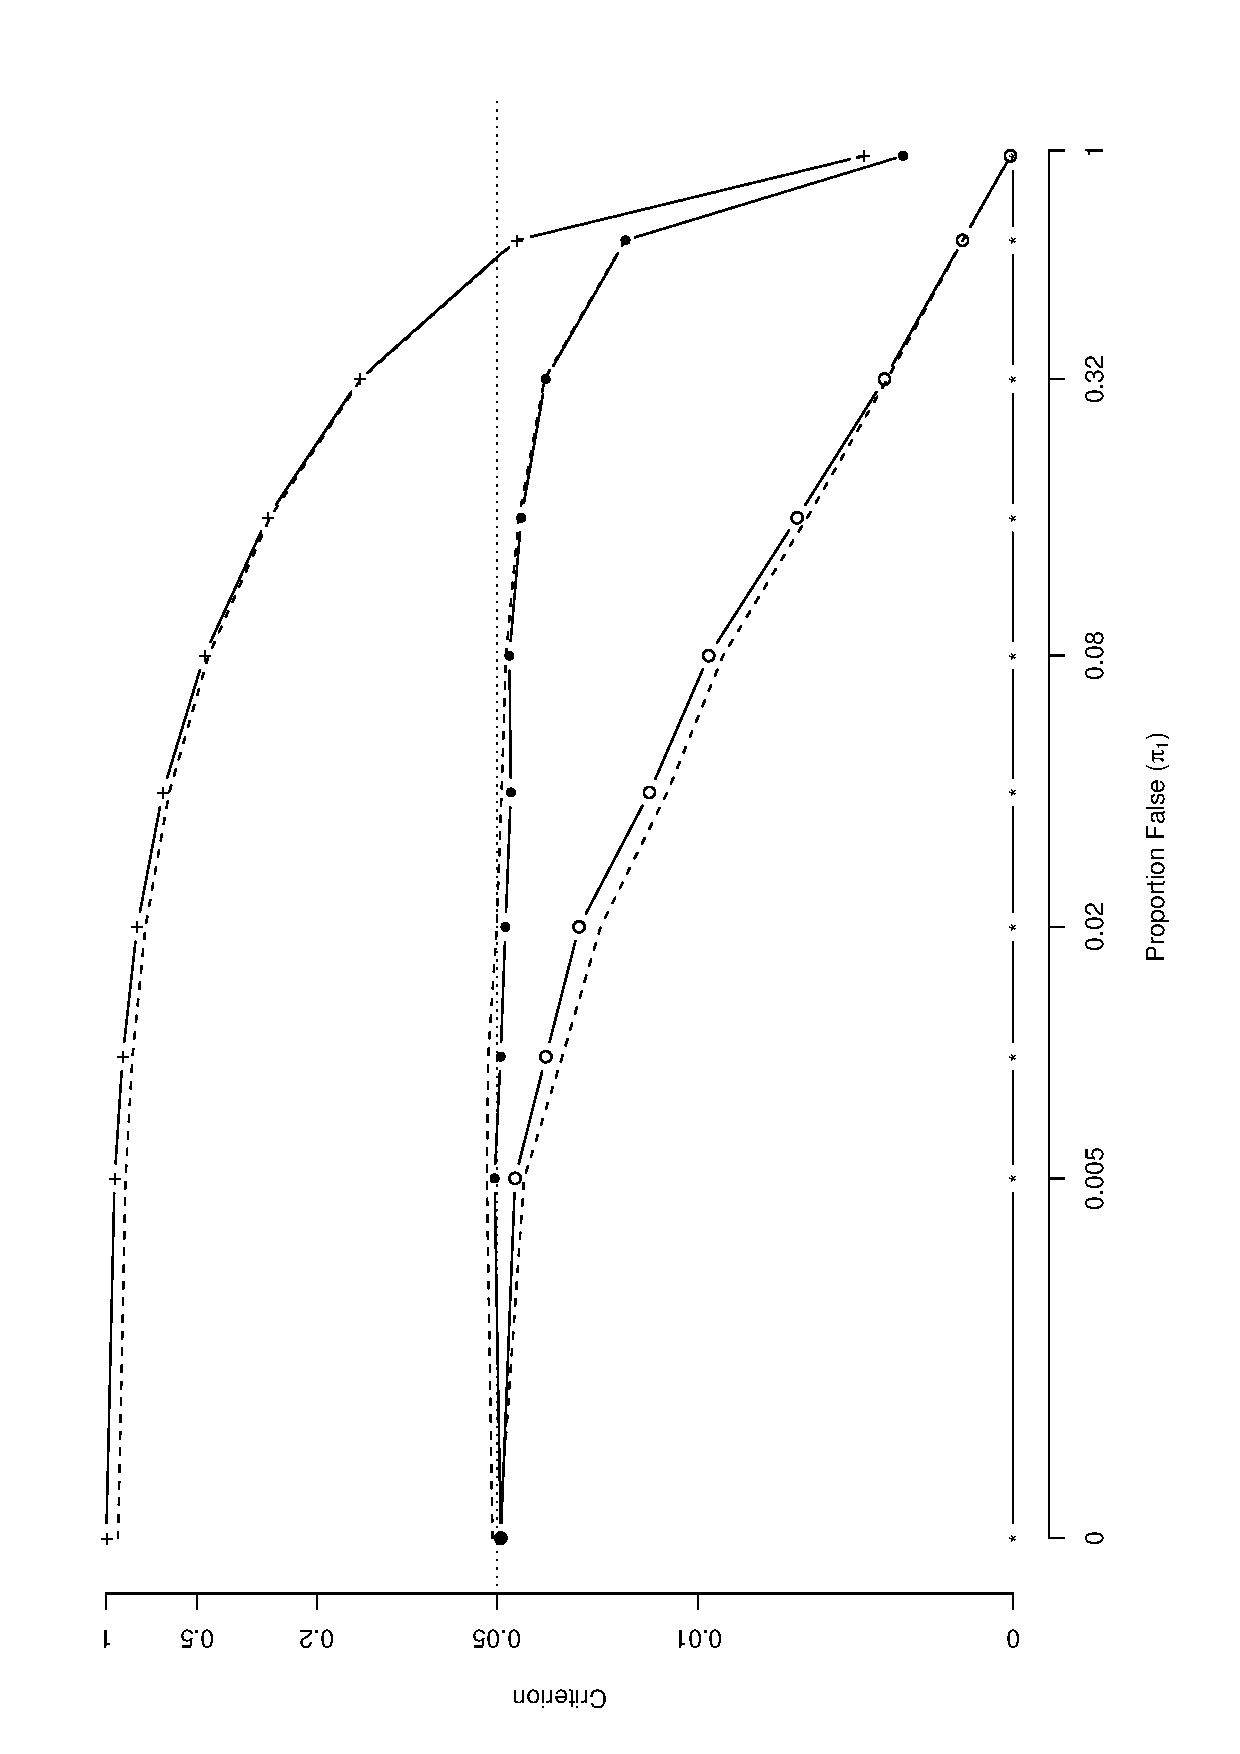
\includegraphics[width=4in]{figure1}  }
\end{figure}


Figure \ref{fi:fig1} confirms the similarity of control implied by FDR and mFDR.   
Both criteria identify the failure of naive testing; FDR and mFDR
 approach 1 unless $\pi_1$ approaches 1.  
The criteria also provide similar assessments of the other
 two procedures; Bonferroni and step-down testing control 
 FDR and mFDR for all levels of signal.  As $\pi_1$ increases and 
 more hypotheses are rejected, both FDR and mFDR of all procedures fall toward zero.   
 The FDR of the wBH procedure is identically zero because it
  only tests false null hypotheses and cannot incorrectly reject a hypothesis.

%--------------------------------------------------------------------------
\section{Uniform control of mFDR}      \label{sec:sFDR}    % 5
%--------------------------------------------------------------------------

Because alpha-investing proceeds sequentially, the testing can
 halt after some number of rejected hypotheses. To control such
 sequential testing, we extend the definition of $mFDR_\eta(m)$ 
 to random stopping times.  
 Recall the definition of a stopping time: $T$ is a stopping  time
  if the event $T \le j$ can be determined by information known 
  when the $j$th test is completed.  

\begin{definition}
 If  $T$ denotes a finite stopping time of a procedure for testing a 
 stream of hypotheses $H_1,\,H_2,\, \ldots$ then
\begin{displaymath}
  \mbox{mFDR}_\eta(T) 
   = \sup_{\theta \in \Theta} \; \frac{E_\theta \left(V^\theta(T)\right)}
                                              {E_\theta \left(R(T) \right) + \eta }\;.
\end{displaymath}
\end{definition}

\noindent 
The supremum over stopping times of mFDR  determines the uniform mFDR:

\begin{definition}
A testing procedure provides {\em uniform control} of mFDR$_\eta$ at level $\alpha$ if 
\begin{equation}
\forall(T \in {\cal T}) \,\,  \mbox{mFDR}_\eta(T) \le \alpha
\label{eq:def:sFDR}
\end{equation}
where ${\cal T}$ is the set of finite stopping times.
\end{definition}

Before proving that alpha-investing provides uniform
 control of mFDR, we prove half of theorem \ref{thm:stopped}.  
 We first define the relevant stopping time.
\begin{definition}
The stopping time $T_{R=r} \equiv \inf_{t}\{t|R(t) = r\}$ where
 we take $T_{R=r}$ to be $\infty$ if the set is empty.
\end{definition}

\begin{lemma}
For any testing procedure that uniformly controls mFDR$_\alpha$ 
at level $\alpha$,
\begin{displaymath}
   E _\theta\; V^\theta(T_{R=r}) \le \alpha (r + 1 - \alpha) \;. 
\end{displaymath}
\end{lemma}

\noindent {\bf Proof.}
Let $\tau \ge 1$ denote an arbitrary, but finite, number of tests.  
We can stop the process at $T \equiv T_{R=r} \wedge \tau$ to make it
 a finite stopping time. Thus $E_\theta(R(T)) \le r$.  We know by
 our hypothesis $E_\theta ( V^\theta(T)) \le \alpha \left({E_\theta(R(T) ) +
 1 - \alpha }\right) =  \alpha(r+ 1 - \alpha)$.  Since this holds for all $\tau$ and
 $V^\theta(t)$ is bounded by $r$, we can take the limit as $r$ increases.

\hfill \QED

mFDR and a variety of modifications of FDR become equivalent 
when stopped at a fixed number of rejections. A bit of algebra shows that
\begin{equation}
-\gamma_R^2 \le \hbox{mFDR}_0 -  \hbox{FDR} -  \gamma_R \frac{\rho \sigma_V}{\mu_R} \le 0
\;,
\label{eq:bounds}
\end{equation}
where $\mu_V$ and $\sigma_V$ are the mean and standard deviation, respectively, of $V^\theta(j)$, the coefficient of variation $\gamma_R = \sigma_R/\mu_R$, and $\rho$ is the correlation
 between $V^\theta(j)$ and $R(j)$.  When $\gamma_R$ is small, FDR and mFDR${}_0$ are close.
If $T_{R=r}$ is finite almost surely, then the standard deviation of
$R$ is identically zero, and hence $\gamma_R = 0$.  So, mFDR${}_0$ and FDR
are identical. The following theorem is similar in spirit to \cite{thc03} who work in a Bayesian setting.
\begin{theorem}\label{thm:all:same}
Suppose $T_{R=r} < \infty$ almost surely.  Then a testing procedure that
 stops when $r$ rejections have occurred has the following properties:
\begin{enumerate}
\item $\gamma_R = 0$.
\item FDR = mFDR${}_0$ = cFDR = eFDR = pFDR = $E\,(V^\theta(r))/r$.
\item FDR $ \le \alpha \frac{r + 2}{r + 1}$ if the procedure has
uniform control of $mFDR_{0}$ at level $\alpha$.
\end{enumerate}
Further, for alpha-investing rules with $\alpha = \omega = W(0) $, then
\begin{enumerate}\setcounter{enumi}{3}
\item $\Var(V^\theta(r)) \le \alpha \, r$.
\item \label{itm:martingale} $P(V^\theta(r) \ge 1 + \alpha \, r + k\sqrt{r}) \le e^{-k^2/2}$.
\end{enumerate}
\end{theorem}
\noindent
The proofs of all five results are straightforward and hence omitted. Property \ref{itm:martingale} has a relationship to \citet{wasserman02, wasserman04}.  In \citet{wasserman04} a stochastic process of
 hypothesis tests is considered.  Their approach contrasts with ours
 in that they use a stochastic process indexed by p-values, whereas we
 use a process indexed by the {\it a priori} order in which hypotheses are 
 considered.  In both cases, an appropriate martingale
 converts expectations into tail probabilities.


The following theorem shows that an alpha-investing rule ${\cal
 I}_{W(0)}$ with wealth determined by \eqn{eq:Wm} controls
 mFDR${}_{1-W(0)}$ so long as the pay-out $\omega$ is not too large.
  The theorem follows by showing that a stochastic process related to
 the alpha-wealth sequence $W(0), W(1), \ldots$ is a sub-martingale.
  Because the proof of this result relies only on the optional
 stopping theorem for martingales, we do not require independent
 tests, though this is the the easiest context in which to
 show that the p-values are honest in the sense required for
 \eqn{eq:alpham} to hold.

\begin{theorem} \label{th:main} An alpha-investing rule ${\cal
 I}_{W(0)}$ governed by \eqn{eq:Wm} with initial alpha-wealth
 $W(0) \le \alpha \, \eta$ and pay-out $\omega \le \alpha$ controls
 mFDR$_\eta$ at level $\alpha$.
\label{eq:theorem1}
\end{theorem}
Theorem \ref{th:main} also applies to the stopped version of mFDR and
 hence shows uniform control.  A proof of this theorem is in the
 appendix.


\paragraph{Remark.} 
It may not be obvious that the condition of a finite stopping time
 $T_{R=r} < \infty$ can in
 fact be met. Given an infinite sequence of hypotheses, define 
 $S^\theta(\infty) = \lim_{m \to \infty} S^\theta(m)$. 
If $S^\theta(\infty) = \infty$ then $T_{R=r} < \infty$ for all $r$ because
 $R(m) \ge S^\theta(m)$.   A parameter $\theta$ 
 that has the property (for all $m$ and all $W(m) > 0$) that
 the chance that the alpha-investing procedure $\cal I$ will reject at
 least one more hypothesis after $m$ is at least $0.5$ is said to
provide  {\em continuous funding} for $\cal I$.  Clearly for such a
 $\theta$ we have that $S^\theta(\infty) = \infty$.

We say that an alpha-investing procedure is {\em thrifty} if it
 never commits all of its current alpha-wealth to the current hypothesis. An
  alpha-investing procedure is {\em hopeful} if it
 always spends  some  wealth on the next hypothesis.  A
 hopeful, thrifty procedure consumes some of its alpha-wealth to test
 every hypothesis in an infinite sequence. With these preliminaries, it
 can be shown that
 % \begin{theorem} \label{thm:finite:stopping}
for any hopeful, thrifty alpha-investing procedure there exists a
distribution $P_\theta$ that provides continuous funding so that $T_{R=r}$
is finite almost surely.
% \end{theorem}


%--------------------------------------------------------------------------
\section{Examples}              \label{sec:examples}           %  6  
%--------------------------------------------------------------------------

This section discusses practical issues of using 
 alpha-investing.  We start by offering general guidelines, or policies,
 on how to construct alpha-investing rules. An example constructs an 
 alpha-investing rule that mimics step-down testing. We conclude with
 simulations that show the advantages of a good policy and compare
 alpha-investing to BH procedures.

Alpha-investing allows the statistician to incorporate prior beliefs
 into the design of the testing procedure while avoiding
 the quagmire of uncorrected multiplicities.  This flexibility
 opens the question of how such choices should be made.
 We can recommend a few policies.  

\begin{description}
\item{\bf Best-foot-forward policy.}
 Ideally, the initial hypotheses include those believed most likely to be
 rejected.  For example, in a testing drugs, it is common to
 test the primary endpoint before others. Alpha-investing rewards this approach: 
 the rejection of the leading hypotheses earns additional alpha-wealth toward tests 
 of secondary endpoints.
 
\item{\bf Spending-rate policies.} Compared to ordering the 
 hypotheses, deciding how much alpha-wealth to spend on each is 
 less important. That said, spending too slowly is inefficient.  
 There is no reward for conserving alpha-wealth unused; the procedure 
 could have used more powerful tests. Alternatively, spending too quickly  may 
 exhaust the alpha-wealth before testing every hypothesis.  It seems reasonable 
 to use a thrifty procedure that reserves some alpha-wealth for future tests.  

\item{\bf Dynamic-ordering policies.} Suppose you are lucky enough to have a
 drug that might cure cancer {\em and} heart disease.  Clearly, these two
 hypotheses should be tested first.  But what should come next
 if the procedure rejects one but not the other? The entire collection of subsequent tests depends on which of the initial hypotheses has been rejected.  The nature of such dynamic-ordering policies is clearly domain-specific. 

\item{\bf Revisiting policies.} Our theorems make no assumptions on how 
 the various hypothesis are related.  This flexibility makes it possible to test  
 hypotheses that closely resemble others.  In fact, our theorems
 hold if the {\em same} hypothesis is tested more than once, so long as
 subsequent tests  condition on prior outcomes.  
 For example, it might be sensible to test $H_{j}$
 initially at a small level $\alpha_{j} = 0.001$ (so as not to risk much alpha-wealth) 
 and then test other hypotheses. If the test does not
 reject $H_j$ the first time, it might make sense to test this hypothesis
 again at a higher level, say, 0.01.  In this way, the procedure distributes
  its alpha-wealth among a variety of
 hypotheses -- spending a little here and then a little there. 
\end{description}


The following testing procedure illustrates how alpha-investing benefits when
 the investigator has accurate knowledge of the underlying science. 
 If the investigator can order
 hypotheses {\it a priori} so that the procedure first tests those most likely to
 be rejected (best-foot-forward policy), then
 alpha-investing rejects more hypotheses than the step-down 
 test of BH.  The full benefit is only realized, 
 however, when combined with a spending-rate policy. 
Suppose that the test procedure has rejected $H_{k^{*}}$ and is about to
test $H_{k^{*}+1}$.  Rather than spread its current alpha-wealth
$W(k^{*})$ evenly over the remaining hypotheses,  allocate
$W(k^{*})$ using a discrete probability mass function such as the following
version of  \eqn{eq:I-sqr}.  This version consumes all remaining alpha-wealth by the
last hypothesis by setting
\begin{equation}
\alpha_j =  \;W(j-1)\left(\frac{1}{1 + j-k^{*}} \vee \frac{1}{1 + m - j}\right)
\label{eq:aggressive}
\end{equation}
If a subsequent test rejects a hypothesis, the procedure reallocates
 its wealth so that all is spent by the time the procedure tests
 $H_m$.  Mimicking the language of financial investing, we describe
 this type of alpha-investing rule as {\it aggressive}.
 
 
In the absence of domain knowledge, a revisiting policy produces an 
 alpha-investing rule that imitates the step-down BH procedure. Begin
 by investing small amounts of alpha-wealth in the initial test of
 every hypothesis.  This conservative policy means that the procedure
 runs out of hypotheses well before it runs out of alpha-wealth.  To
 improve its power, the rule uses its remaining alpha-wealth to
 take a second pass through the hypotheses that were not rejected in
 the first pass.  Although we do not advocate this as a general
 procedure, it is allowed by our theorems.  Gradually ``nibbling''
 away at the hypotheses in this fashion results in a procedure that resembles
  step-down testing.  In fact, as the size of
 these nibbles goes to zero, the order that hypotheses are rejected is
 precisely that from step-down testing.  The point where each testing procedure
 stops is slightly different.  Sometimes step-down testing stops first and
 sometimes alpha-spending stops first.

A few calculations clarify the connection to the BH procedure. To avoid taking many passes through the hypotheses without generating
 any rejects, increase the size of the nibbles so as to take as large a bite each time
 as possible.  Set $\alpha = \omega = W(0)$.  The
 procedure begins by testing each hypothesis in ${\cal H}(m)$ at level
 $\beta_{1} = \al/(\al + m) \approx \al/m$, approximating the
 Bonferroni level.  This  level assures us that the
 procedure exhausts its alpha-wealth if no hypothesis is
 rejected.  If, however, some hypothesis is rejected, the procedure
 uses the earned alpha-wealth to revisit the hypotheses that were not
 rejected in the first pass.  At the start of each pass, the algorithm
 divides its alpha-wealth equally among all remaining unrejected hypotheses
 and tests each at this common level.  These steps continue 
 until a pass  does not reject a hypothesis and the 
 alpha-wealth reaches zero. 
 
 On successive passes through the hypotheses, the
 fact that a hypothesis was previously tested must be used in
 computing the rejection region.  Suppose that
 exactly one hypothesis is rejected at each pass.  In the first pass, 
  the p-value of one hypothesis is smaller than the initial level $\beta_{1}$.
  Following \eqn{eq:Wm}, the rule pays $\beta_{1}/(1-\beta_{1})$ for
 each test that it does not reject and earns $\al$ for rejecting
 $H_{(1)}$.  Hence, after the initial test of each hypothesis at level
 $\beta_{1}$, the alpha-wealth grows slightly to
\begin{eqnarray}
 W(m) 
   &=& W(0) + \omega - (m-1) \beta_{1}/(1-\beta_{1})      \cr
   &=& \alpha + \al/m               
\label{eq:approx}
\end{eqnarray}
For large $m$, its alpha-wealth is virtually unchanged from $W(0)$.

For the second pass, the procedure again distributes
 its alpha-wealth equally over the remaining hypotheses.  
 The level invested in each test at this second pass is
\begin{displaymath}
  \beta_2 = \frac{W(m)}{W(m)+m-1} > \frac{\al}{m} \;.
\end{displaymath}
To determine which tests are rejected during the second pass, assume that
 the remaining p-values are uniformly distributed.  Conditioning on
 $p_j > \beta_1$, this pass rejects any hypothesis for which $p_j \le
 p^{*}$ with the threshold $p^{*}$ determined by
\begin{displaymath}
  \pr_0\left(
   p_j \le p^{*} \given p_j > \beta_1 
    \right) =  \frac{p^{*} - \beta_1}{1-\beta_1} = \beta_2 \;.
\end{displaymath}
This implies that $p^{*} = \beta_1+\beta_2 - \beta_1\beta_2 \approx 2
 \al/m$. Thus, the second pass approximately rejects any hypotheses
 with p-value is smaller than $2\,\al/m$, the second threshold of the
 step-down test.  In this way, the investing rule gradually raises the
 threshold for rejecting hypotheses as in step-down testing.  If any
 hypothesis is rejected during a pass over the remaining hypotheses,
 then alpha-wealth remains and the testing procedure continues
 recursively. Instead of spending equally on each hypothesis one could
 weight these hypotheses differently.  This idea of using prior
 information is implicit in alpha-spending rules. The use of prior
 information also appears in the wBH procedure proposed in
 \cite{wasserman06}.  Following the ideas of this section, we can show
 that the wBH procedure controls mFDR.

 \vspace{0.1in} {\noindent}{\bf Simulations.} Our first simulation
 compares three alpha-investing rules to step-down versions of the BH
 and wBH procedures. As in Section 3 for the wBH procedure, an oracle
 assigns weights
\begin{displaymath}
    W_j = \left\{ \begin{array}{cc}
                   0                     & \mbox{ if } H_j \mbox{ is true } \cr
                   1/S^\theta(m) & \mbox{ otherwise, }
               \end{array} \right.
\end{displaymath}
to each hypothesis so that wBH only tests false hypotheses. For the
 sake of comparison, each replication of the simulation tests a fixed
 batch of $m = 200$ hypotheses.  The 200 hypotheses are defined as in
 the simulation in Section 3 (see equation \ref{eq:mu-j}); this
 simulation also uses 10,000 samples. Of the alpha-investing rules,
 one implements the revisiting policy that mimics the BH procedure.
  The other two alpha-investing rules implement aggressive
 alpha-investing. To illustrate the impact of domain knowledge, we
 simulated the performance of alpha-investing using
 \eqn{eq:aggressive} in a best-case and a worst-case scenario.  For
 the best case, the investigator tests the hypotheses in the order
 implied by $|\mu_j|$, testing the hypothesis with the largest
 $|\mu_j|$ first. The tests are ordered by the underlying means rather
 than the observed p-values.  In the worst case, the hypotheses are
 tested in random order, indicating poor domain knowledge. We set the
 level for all procedures to $\al = 0.05$; for alpha-investing, the
 initial wealth $W(0) = \alpha = \omega$ and $\eta= 1-\alpha$.
 
Figure \ref{fi:fig2}(a) shows the FDR of each procedure. As in the
 prior simulation summarized in Figure \ref{fi:fig1}, FDR and mFDR are
 quite similar in this simulation and so we have only shown FDR.  All
 five procedures control FDR (and mFDR), as they should. As in Figure
 \ref{fi:fig1}, the FDR of the wBH procedure is identically zero
 because it tests only false null hypotheses. For the other procedures
 that do not benefit from this oracle, it becomes easier to control
 FDR in the presence of more false null hypotheses (larger
 $\pi_1$). Accurate domain knowledge reduces the FDR of the aggressive
 procedure. When tested in random order (poor domain knowledge), the
 FDR of aggressive testing is similar to that of the BH step-down
 procedure.
 

\begin{figure}
\caption{     \label{fi:fig2} \sl
Comparison of the FDR and power of aggressive alpha-investing rules with accurate ($\triangledown$) and inaccurate ($\vartriangle$) domain knowledge to BH ($\bullet$), oracle-based wBH ($\star$), and a revisiting alpha-investing rule ($\circ$).  (a) All five procedures control FDR. (b) Better domain knowledge improves the power of alpha-investing relative to step-down testing. The vertical axis shows the ratio of the number of correctly rejected null hypotheses relative to BH.
}
\centerline{ 	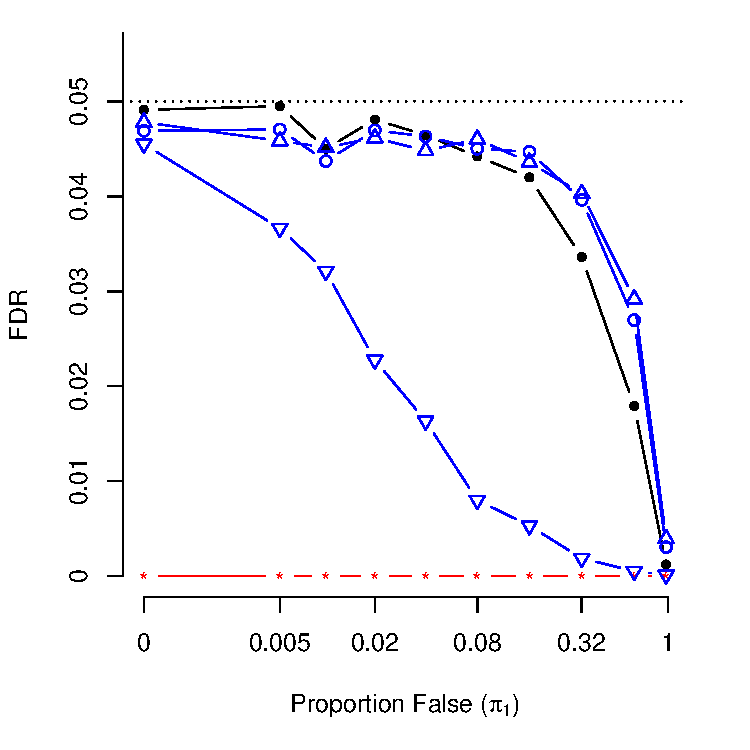
\includegraphics[width=3in]{figure2a}
			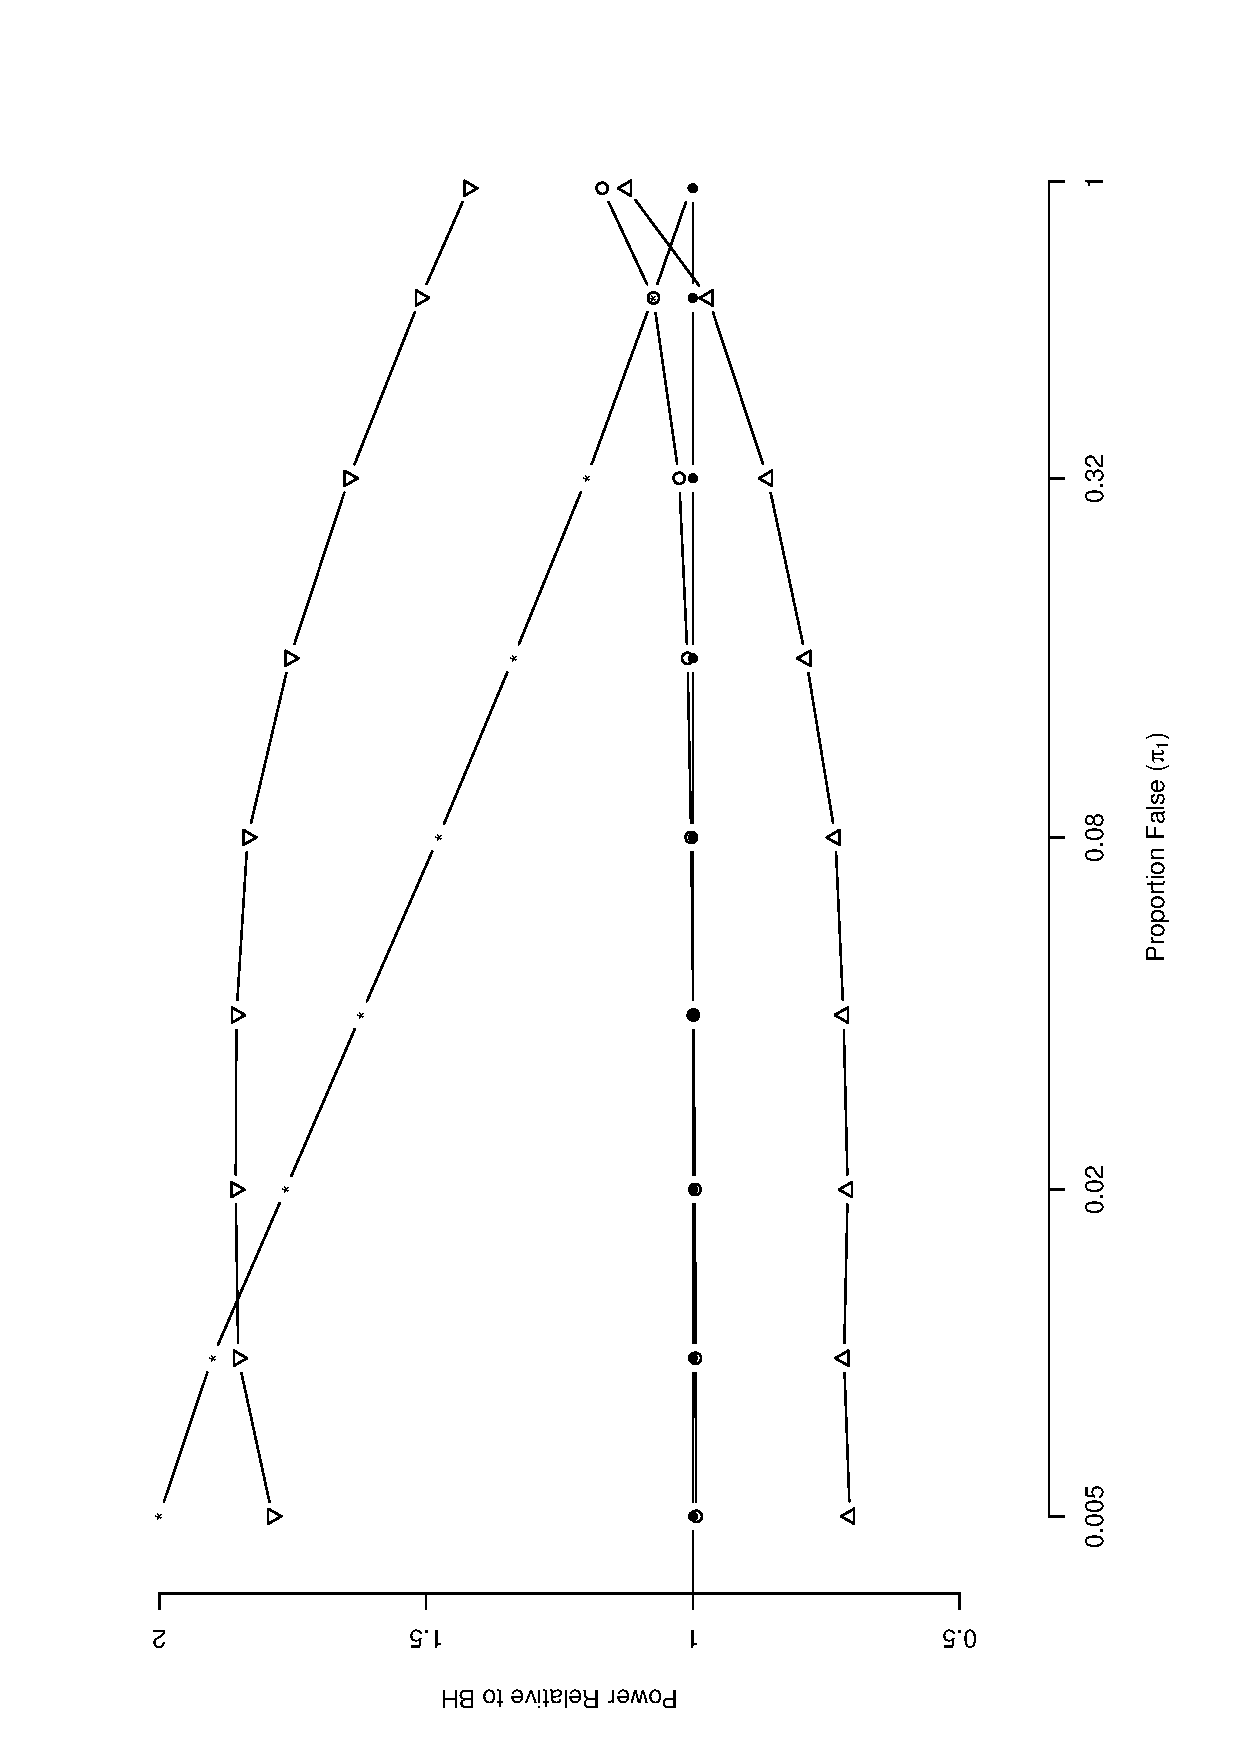
\includegraphics[width=3in]{figure2b}   }
\end{figure}


Alpha-investing guarantees protection from too many false rejections,
but how well does it find signal?  For each alpha-investing rule, Figure \ref{fi:fig2}(b)
shows the ratio of the number of correctly rejected hypotheses relative to the number rejected by BH, estimating
\begin{displaymath}
E_\theta\, \left( \frac{S^\theta(200,\mbox{test procedure})}
                       {S^\theta(200,\mbox{BH})} \right)
\end{displaymath}
from the simulation.  With accurate domain knowledge, aggressive
 alpha-investing rejects in excess of 50\% more hypotheses than the
 step-down BH procedure. Unless the problem offers few false null
 hypotheses ($\pi_1<0.02$, an average of 1 or 2 false null
 hypotheses), aggressive alpha-investing with good domain knowledge
 obtains the greatest power. Alpha-investing gains more from testing
 the hypotheses in the right order than BH gains from knowing which
 hypotheses to test.  If the domain knowledge is poor, aggressive
 alpha-investing rejects no less than 70\% of the number rejected by
 step-down testing.  As expected from its design, alpha-investing
 using the revisiting policy performs similarly to step-down testing.

We also performed a simulation to investigate the performance of
 alpha-investing when applied to an infinite stream of hypotheses.
  Each null hypothesis specifies a mean ($H_t: \mu_t = 0,\, t =
 1,\,2,\,\ldots$), and the test statistic for each hypothesis is $Z_t
 \sim N(\mu_t, 1)$, independently.  The simulation computes the FDR
 and power of aggressive alpha-investing using the rule \eqn{eq:I-sqr}
 and a two-sided test of $H_t$.  Two levels of signal are present in
 the simulation. Under one scenario, 10\% of the null hypotheses are
 false; in the second, 20\% are false.  For each scenario, false null
 hypotheses cluster in bursts of varying size.  We generated the
 sequence of means $\mu_t$ from a two-state Markov chain $\{Y_t\}$.
  In state 0, the null hypothesis holds, $\mu_t = 0$.  In state 1,
 $\mu_t = 3$.  The transition probabilities for the Markov chain are
 $p_{ij} = P(Y_{t+1} = j \given Y_{t}=i)$. The probability of leaving
 state 0 varies over $p_{01} = (0.0025, 0.005, 0.010, 0.025, 0.05)$.
  To obtain a fixed percentage of false null hypotheses, we set
 $p_{10} = k \, p_{01}$ with $k = 4$ (20\% false null hypotheses) and
 $k=9$ (10\%). Given $k$, increases in the transition probability
 $p_{01}$ produce a more choppy sequence of hypotheses. We simulated
 1,000 streams of hypotheses for each combination of $k$ and $p_{01}$,
 beginning each with $Y_1=1$ (a false null). As in previous
 simulations, we set $W(0) = \alpha = \omega = 0.05$ and $\eta=
 1-\alpha$.

Figure \ref{fi:stream} presents a snapshot of the results after
 testing 4,000 hypotheses. Although aggressive alpha-investing is
 thrifty and hopeful in the sense of Section 5, it can be shown that
 the sequence of means $\{\mu_t\}$ generated by the Markov chain do
 not provide continuous funding.  Each sequence of tests eventually
 stops after a finite number of tests when the alpha-wealth runs out.
  Even so, at the point of the snapshot in Figure \ref{fi:stream},
 each simulated realization of alpha-investing has enough alpha-wealth
 to reject further hypotheses. For example, the retained alpha-wealth
 $W(4000)$ averaged 0.003 with $k=9$ and $p_{01} = 0.05$ (fewest, most
 choppy false hypotheses) up to 0.63 with $k=4$ and $p_{01} = 0.0025$.
  In every case, Figure \ref{fi:stream}(a) shows that the FDR lies
 well below 0.05.

Figure \ref{fi:stream}(b) shows that aggressive alpha-investing has
 higher power when applied to sequences with a higher proportion of
 false null hypotheses that arrive in longer clusters. This situation
 affords the best opportunity to accumulate alpha-wealth that can be
 spent quickly to reject clustered false hypotheses. The power rises
 rapidly once a cluster of false null hypotheses is discovered. For
 example, the overall power is 0.51 with $k=4$ and $p_{01} = 0.025$
 (20\% false nulls with mean cluster size 10).  For finding the first
 null hypothesis of each cluster, however, the power falls to 0.20.
  This observation suggests that a revisiting policy that returns to
 hypotheses immediately preceding a rejected hypothesis would have
 higher power. In general, the power shown in Figure
 \ref{fi:stream}(b) rises roughly linearly in the log of the mean
 cluster size $1/p_{10}$. Aggressive alpha-investing also finds a
 higher percentage of the false null hypotheses when more are present.
  The power is consistently higher when 20\% of the hypotheses are
 false ($k$ = 4) than when 10\% are false ($k$ = 9). The gap between
 these scenarios diminishes slightly as the mean cluster size
 increases. As in the prior simulation, the higher power obtained for
 longer clusters is accompanied by smaller rates of false discoveries.

\begin{figure}
\caption{     \label{fi:stream} \sl
The power of aggressive alpha-investing increases with a higher proportion of false null hypotheses that arrive in longer clusters. The frames show (a) FDR after completing 4,000 tests and (b) power ($\circ$ denotes 10\% false nulls ($k=9$) and $\times$, 20\% false nulls  ($k=4$)).
}
\centerline{ 	
	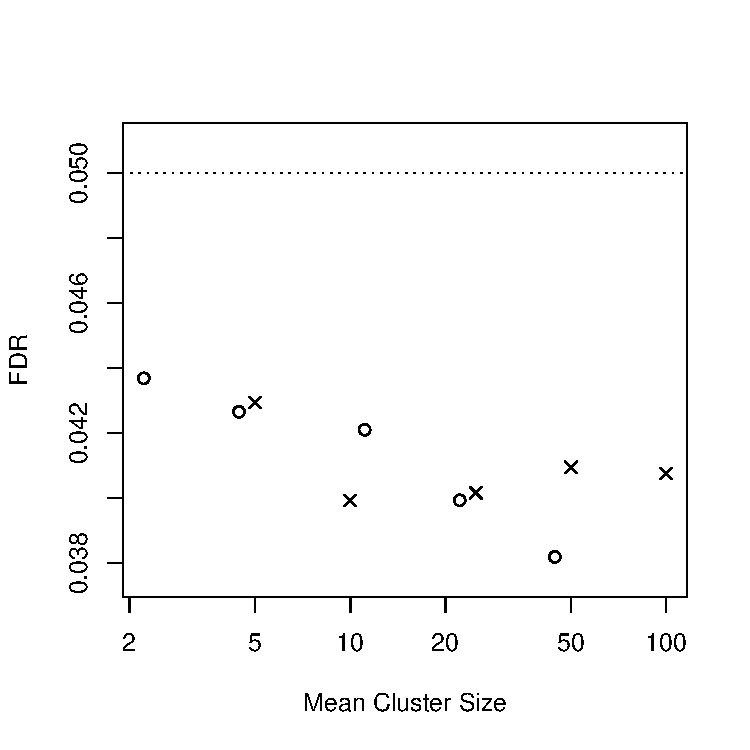
\includegraphics[width=3in]{figure3a}  
	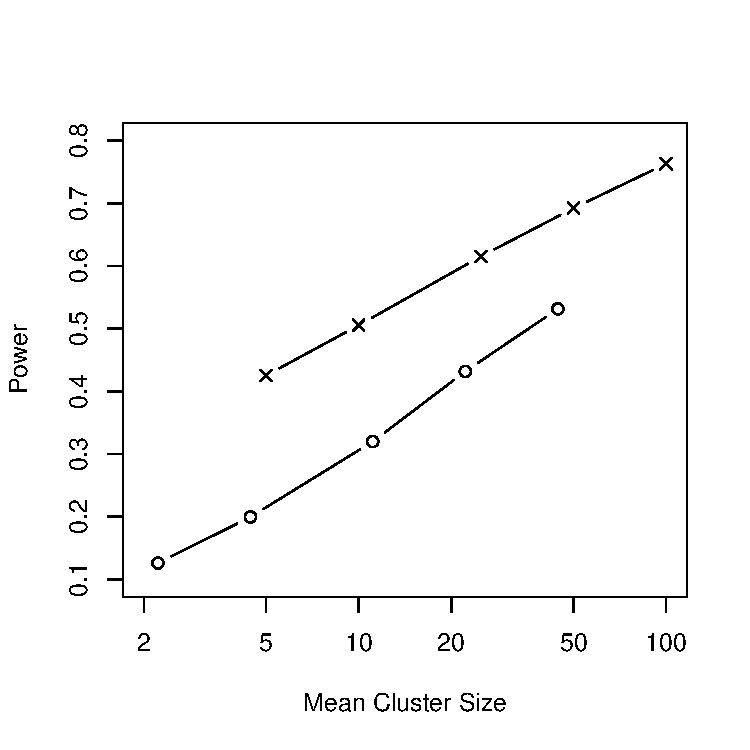
\includegraphics[width=3in]{figure3b}
	 }
\end{figure}



%--------------------------------------------------------------------------
\section{Discussion}           \label{sec:discussion}
%--------------------------------------------------------------------------

The best-foot-forward policy raises a concern relevant to any multiple testing procedure that controls an FDR-like criterion.  Suppose that ${\cal H}(m)$ is contaminated with
 trivially-false hypotheses that artificially produce alpha-wealth. Then all 
 subsequent tests are tainted. As an extreme example, suppose the
  first hypothesis claims  ``gravity does not exist.''  After rejecting this
 hypothesis, the testing procedure has more alpha-wealth to use 
 in subsequent tests than allocated by $W(0)$.  
 Most readers would, however, be uncomfortable
  using this additional alpha-wealth to test the primary endpoint of a drug. 
   As discussed by \citet{finner01}, step-down tests share this problem. By rejecting the trivially false $H_1$, the level of the test of the first ``real hypothesis'' is $2\alpha/m$ rather than $\alpha/m$. In this sense, it is important to allow
an observer to ignore the list of tested hypotheses from some point onward. The design of the sequential test procedure should put the most interesting 
hypotheses first to insure that that when the reader stops, they have seen 
the most important results. By providing uniform control of mFDR, alpha-investing controls this criterion wherever the observer stops.
  

One can regulate alpha-investing using other methods of compensating, or charging, for each test.  The increment in the alpha-wealth defined in \eqn{eq:Wm} is natural,
 with a fixed reward 
 and penalty determined by whether the test rejects a hypothesis, say $H_j$.
 Because neither the payout $\omega$ nor the cost $\al/(1-\al)$ 
 reveals $p_j$ (other than to indicate if $p_j \le \al_j$), subsequent
  tests need only condition on the sequence of rejections, $R_1,\ldots,R_j$.
  The following alternative method for regulating alpha-investing has
  the same expected pay-out,  but varies the winnings when the test rejects $H_j$:
\begin{equation}
  W(j) - W(j-1) =
   \left\{ \begin{array}{cc}
                \omega + \log (1-p_j) & \mbox{ if } p_j \le \alpha_j  \;,\cr
                \log(1 - \alpha_j)       & \mbox{ if } p_j > \alpha_j   \;.
           \end{array} \right.
\end{equation}
Alpha-investing governed by this ``regulator'' also satisfies the
theorems shown previously.  Because the reward reveals $p_j$ when $H_j$ is
rejected, however, the investing rule must condition on $p_j$ for any rejected prior
hypotheses.  This would seem to complicate the design of tests in applications in which
the p-values are not independent. Other methods for regulating the alpha-wealth
could be desirable in other situations.  We hope to pursue these ideas in future work.


We speculate that the greatest reward from developing a specialized
testing strategy will come from developing methods that select the
next hypothesis rather than specific functions to determine how $\alpha$
is spent.  The rule \eqn{eq:aggressive} invests half of the current
wealth in testing hypotheses following a rejection.  One can devise other choices. 
Results in information theory 
\citep{rissanen83, fosterstinewyner02}, however, suggest that one can 
find universal alpha-investing rules.  A universal alpha-investing
rule would reject on average as many hypotheses as the best rule
within some class. We would expect such a rule to spend its
alpha-wealth more slowly than the simple rule
\eqn{eq:aggressive}, but retain this general form.


%--------------------------------------------------------------------------
\section*{Appendix}  
%--------------------------------------------------------------------------

\subsection*{Proof of Theorem \ref{th:main}}

We begin by defining a stochastic process indexed by $j$, the
number of hypotheses that have been tested:
\begin{displaymath}
    A(j) \equiv \alpha R(j) -  V^\theta(j)  +  \eta\,\alpha - W(j) \; .  
\end{displaymath}
Our main lemma shows that $A(j)$ is a sub-martingale for
 alpha-investing rules with pay-out $\omega \le \alpha$.  In other
 words we will show that $A(j)$ is ``increasing'' in the sense that
\begin{displaymath}
  E_\theta\left( A(j) \given A(j-1),\,A(j-2),\ldots, A(1)\right)
  \ge A(j-1) \;.
\end{displaymath}
Theorem \ref{th:main} uses the weaker fact that
 $E_\theta A(j) \ge A(0)$.  By definition $V^\theta(0) = R(0) = 0$ so that
 $A(0) = \eta\,\alpha - W(0) \ge 0$ if $W(0) \le
 \eta\,\alpha$.  When $A(j)$ is a sub-martingale, the optional stopping
 theorem implies that for all finite stopping times $M$ that $E_\theta A(M)
 \ge 0$.  Thus,
\begin{eqnarray*}
E_\theta \left(\alpha (R(M)+\eta) - V^\theta(M) \right)
  & =   &  E_\theta \left(W(M) + A(M) \right) \cr
  & \ge& E_\theta \,A(M)               \cr
  & \ge& A(0) \ge 0 \; .
\end{eqnarray*}
The first inequality follows because the alpha-wealth $W(j) \ge 0 \;
 [a.s.]$, and the second inequality follows from the sub-martingale
 property.  Thus, once we have shown that $A(j)$ is a sub-martingale, it follows
 that $E_\theta \, V^\theta(M)  \le  \alpha (E_\theta\,R(M)+\eta)$ and
\begin{displaymath}
  \mbox{mFDR}_\eta(M) = \frac{E_\theta\,V^\theta(M)}{ E_\theta\,R(M)+\eta}  \le   \alpha.
\end{displaymath}
Thus to show Theorem \ref{th:main} we need to prove the following lemma:

\begin{lemma} \label{le:martingale} Let $V^\theta(m)$ and $R(m)$
 denote the cumulative number of false rejections and the cumulative
 number of all rejections, respectively, when testing a sequence of
 null hypotheses $\{H_1,\,H_2,\,\ldots\}$ using an alpha-investing
 rule ${\cal I}_{W(0)}$ with pay-out $\omega \le \alpha$ and
 alpha-wealth $W(m)$.  Then the process
\begin{eqnarray*}
    A(j) 
  &\equiv& \alpha R(j) - V^\theta(j) + \eta \, \alpha  - W(j) 
\end{eqnarray*}
is a sub-martingale,
\begin{equation}
   E_\theta \left(A(m) \given A(m-1), \ldots, A(1)\right) \ge A(m-1) \;.
 \label{eq:super}
\end{equation}
\end{lemma}

\noindent 
{\bf Proof.} 
Write the cumulative counts $V^\theta(m)$ and $R(m)$ as sums of
indicators $V^\theta_j,\, R_j \in \{0,1\}$,
\begin{displaymath}
   V^\theta(m) = \sum_{j=1}^m V^\theta_j \;, \qquad
   R(m) = \sum_{j=1}^m R_j \;.
\label{eq:sums}
\end{displaymath}
Similarly write the accumulated alpha-wealth $W(m)$ and $A(m)$ as sums of
increments, $W(m) = \sum_{j=0}^m W_j$ and $A(m) = \sum_{j=0}^m A_j$.
Let $\alpha_j$ denote the alpha level of the test of $H_j$ that satisfies
the condition \eqn{eq:alpham}.  The change in the alpha-wealth from
testing $H_j$ can be written as:
\begin{displaymath}
  W_j  =  R_j \omega - (1-R_j) \al_j/(1-\al_j)  \;,
\end{displaymath}
Substituting this expression for $W_j$ into the definition of $A_j$ we get
\begin{displaymath}
   A_j  =  (\alpha -\omega) R_j - V^\theta_j  + (1-R_j) \al_j/(1-\al_j) \;.
\end{displaymath}
Since $R_j \ge 0$ and $\alpha - \omega \ge 0$ by the conditions of the
lemma, it follows that
\begin{equation}
\label{eq:a:bound}
A_j  \ge  (1-R_j)\al_j/(1-\al_j) - V^\theta_j   \;.
\end{equation}
If $\theta_j \not\in H_j$, then $V^\theta_j = 0$ and $A_j \ge 0$
almost surely.  So we only need to consider the case in which the null
hypothesis $H_j$ is true. When $H_j$ is true,  $R_j \equiv V_j^\theta$ and 
\eqn{eq:a:bound} becomes
\begin{equation}
\label{eq:a:bound:h0}
A_j  \ge  (1-R_j)\al_j/(1-\al_j) - R_j = (\al_j-R_j)/(1-\al_j)  \;.
\end{equation}
 Abbreviate the conditional expectation
\begin{displaymath}
  E_\theta^{j-1}(X) 
     = E_\theta \left(X \given  A(1),\,A(2),\,\ldots,A(j-1) \right)\;.
\end{displaymath}
Under the null,  $E_\theta^{j-1}\,R_j \le \alpha_j$ by the definition of
this being an $\alpha_j$ level test. Taking conditional expectations in  
\eqn{eq:a:bound:h0} gives $E_\theta^{j-1} A_j  \ge   0$.

\hfill \QED

%--------------------------------------------------------------------------
% References
%--------------------------------------------------------------------------

\bibliography{../stat}
\bibliographystyle{../bst/rss}

\end{document} %==========================================================
